\chapter{Proposed Work}

In this thesis we investigate two questions: ``Does prosthesis control based on
on a dynamic model of the human neuromuscular system generalize better to new
conditions, resulting in a more robust control?'' And ``can we improve the
control behavior by optimizing it's parameters using qualitative feedback from
the amputee?'' To investigate these questions, we propose completing four tasks
before graduation in May 2018: 
\begin{proposed_works} 
    \item[\Cref{sec:proposed_build}] Building and characterizing the performance
    of a prosthesis capable of executing dynamic locomotion tasks.

    \item[\Cref{sec:proposed_evaluate}] Imposing a variety of disturbances to an
    amputee walking on a prosthesis controlled by the Neuromuscular model and
    assessing the recovery response.

    \item[\Cref{sec:proposed_optimize}] Implementing a system to optimize the
    control parameters using qualitative feedback and evaluating its ability to
    improve user satisfaction.

    \item[\Cref{sec:proposed_trip_class}] Improving the existing swing leg
    control by augmenting it with explicit trip detection and execution of
    recovery strategies.
\end{proposed_works} 

\section{Build and Characterize Performance of Transfemoral
Prosthesis}\label{sec:proposed_build}

The first step to addressing these questions is to finish construction of the
prosthesis design presented in \cref{sec:completed_design}. So far we have
built, fabricated, and tested the knee joint and fabricated parts for the ankle.
Remaining tasks include assembly of the parts, improving the wiring and cable
management, and implementing a position-control based series elastic control.
The position based SEA control will command the pre-spring actuator position
$\theta_m$, according to
\begin{align}
    \theta_m = \frac{\tau_d}{k} + \theta_l + \func{PD}{\tau_e} + k_d \omega_l
\end{align}
where $k$ is the series spring stiffness and $k_d \omega_l$ compensates for
damping in the joint. Position based torque control allows the torque control to
take advantage of the fast control loops of our motor controllers (5000 Hz
position control loop versus 1000 Hz Simulink Realtime Control loop). (Compare
to commanding velocity as in the existing control \cref{eq:velocity_based_sea}.)

The preliminary experiments with the active knee joint and passive ankle
prosthesis, shown in
\cref{sec:completed_knee_exp_walk,sec:completed_exp_swing_trip}, suggest the
actuator design seems well suited to the task. However, we have not thoroughly
evaluated the prosthesis performance in terms of step response, bandwidth, and
zero torque tracking. Therefore, we propose to evaluate these characteristics
for both the knee and ankle joints. 

\section{Evaluate Neuromuscular Transfemoral Prosthesis
Control Recovery}\label{sec:proposed_evaluate}

\begin{enumerate}
    \item Evaluate nominal walking gait produced by nm model. Compare to healthy
    walking data in terms of joint kinematics and torque.
    \item investigate ability of control to adapt to different situations:
    \begin{enumerate}
        \item speed adaptation
        \item slope adaptation
        \item sudden treadmill speed change on both sides.
        \item push bot disturbance applied to hip during stance
    \end{enumerate}
    compare to passive prosthesis/impedance control. Evaluate in terms of
    recovery time before returning to normal gait.
\end{enumerate}

\section{Optimizing Prosthesis Control using
Preferences}\label{sec:proposed_optimize}
\begin{enumerate}
    \item Develop simplified acquisition function
    \item incorporate time adaptation, absolute feedback, best ever feedback
    \item perform treadmill gait tuning exp in 1,3, and 5 dimensions (width,
    skewness, frequency, left/right foot direction)
    \item optimize prosthesis control and compare to default params and passive
    prosthesis if amputee subject.
\end{enumerate}

\section{Learning Trip Recovery Policies}\label{sec:proposed_trip_class}
\begin{enumerate}
    \item Implement SVM trip detection and classification on prosthesis.
    \item Use Dagger training method to see if online error rate can be reduced.
\end{enumerate}

\section{Proposed Work Summary and Timeline}\label{sec:proposed_summary}
\begin{figure*}[t]
    \centering
    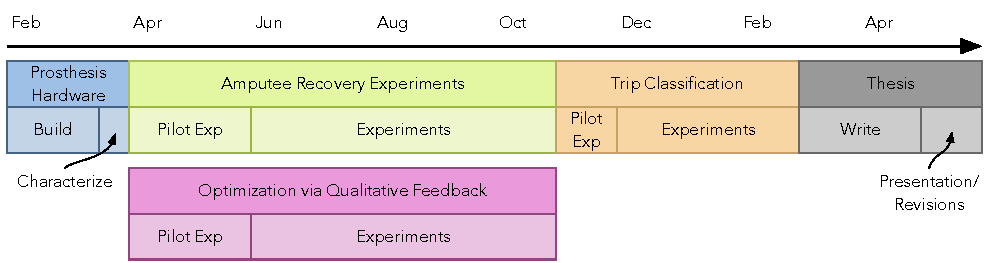
\includegraphics[width=\textwidth]{gantt_chart}
    \caption{Proposed timeline for remaining work.}\label{fig:prosthesis_result}
\end{figure*}
